\scanpage{17}
endomorphisme de $X$, qui n'est d'ailleurs autre que
$(\operatorname{Frob}_S^\nu(X))^k$, comme on constate aussitôt.

D'ailleurs, dans le cas où $\unsure{h|\nu}=1$, i.e.
sur la base absolue $\mathbf Z/p\mathbf Z$, on trouve que
$\operatorname{Frob}_{\mathbf Z/p\mathbf Z}(X)$ est le Frobenius absolu du début.

\uline{Corollaire} Si $S$ est sur $\mathbf F_q$, et si $X$ provient d'un
\unsure{schéma} \deleted{\unsure{sur}} $\mathbf F_q$ \uline{par extension} de la base...
\figure{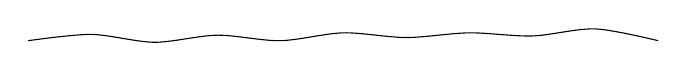
\begin{tikzpicture}\draw plot[smooth] coordinates {(0,0) (.8,.08) (1.6,-.02) (2.4,.07) (3.2,0) (4,.1) (4.8,.04) (5.6,.1) (6.4,.06) (7.2,.15) (8,0)};\end{tikzpicture}}

\uline{Cas des groupes}. Si $G$ est muni d'une
structure algébrique définie sur $S$, il en est
de même de $p_S(G)$, et \deleted{$\operatorname{Frob}_S(X)$}
\[
\operatorname{Frob}_S^\nu(G):G\longrightarrow p_S^\nu(G)
\]
est un morphisme pour les structures en question.
Considérons son noyau, noté
\[
U_\nu(G)=\operatorname{Ker}(\operatorname{Frob}_S^\nu(G)).
\]
\margin{C'est le plus grand sous-schéma en groupes $U\unsure{\subset}G$
pour lequel $\operatorname{Frob}^{\nu}\mathrm{abs}$ est \unsure{trivial}.}
\deleted{\uline{Proposition} Si $G$ est de présentation finie sur $S$, alors
\unsure{?} $U_\nu(G)$ est de présentation finie et \deleted{\unsure{de}}
fini \deleted{\unsure{un}} radiciel \inserted{(surjectif)} sur $S$.}
\mspage{16}
